\section{D\'eterminer la m\'ethode de d\'etermination de valeurs}
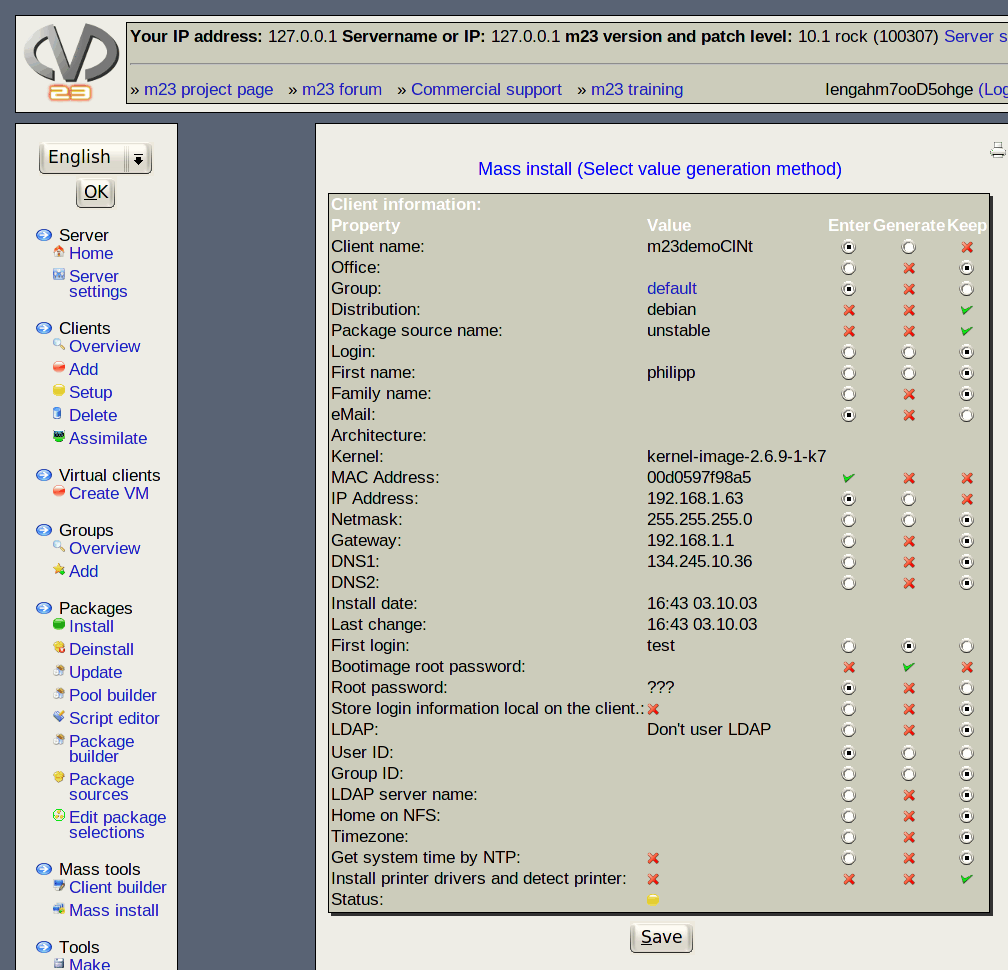
\includegraphics[scale=0.4]{/mdk/doc/manual/screenshots/fr/mi_step0.png} \\
Ici, vous pouvez d\'eterminer comment les valeurs des propri\'et\'es des clients doivent \^etre g\'en\'er\'ees. \\
\subsection{Vous pouvez choisir entre trois m\'ethodes:}
\begin{itemize}
\item \textbf{Entrer}: Vous entrez les propri\'et\'es \`a la main ou par un fichier.\\
\item \textbf{G�n�rer}: Les valeurs seront g\'en\'er\'ees automatiquement. Par exemple, les noms des postes client peuvent \^etre g\'en\'er\'es avec des num\'eros d'ordre ou des adresses IP libre seront utilis\'es.\\
\item \textbf{Garder}: La valeur d\'etermin\'ee pour le $\ll$poste client mod\`ele$\gg$ sera gard\'ee pour tous les postes client.\\
Chez certaines propri\'et\'es, votre choix est limit\'ee. Les m\'ethodes que vous ne pouvez pas choisir sont marqu\'ees avec une croix rouge. Un crochet vert signifie que c'est la seule m\'ethode de d\'etermination de valeurs possible. Par exemple, une adresse MAC ne peut pas \^etre g\'en\'er\'ee, ni \^etre la m\^eme pour tous les postes client. Elle doit \^etre entr\'ee \`a la main ou charg\'ee d'un fichier.\\
\end{itemize}
